\section{\palm algorithm}
\label{sec:app:palm4msa}

The \palm algorithm~\cite{LeMagoarou2016Flexible} is given in Algorithm~\ref{algo:palm4msa} together with the time complexity of each line, using $A=\min(\nclusters, \datadim)$ and $B=\max(\nclusters, \datadim)$. 
Even more general constraints can be used, the constraint sets $\mathcal{E}_q$ are typically defined as the intersection of the set of unit Frobenius-norm matrices and of a set of sparse matrices.
The unit Frobenius norm is used together with the $\lambda$ factor to avoid a scaling indeterminacy.
Note that to simplify the model presentation, factor $\lambda$ is used internally in \palm and is integrated in factor $\rmS_1$ at the end of the algorithm (Line~\ref{line:palm:postprocess:S1}) so that $\rmS_1$ does not satisfy the unit Frobenius norm in $\mathcal{E}_1$ at the end of the algorithm.
The sparse constraints we used, as in~\cite{LeMagoarou2016Flexible}, consist of trying to have a given number of non-zero coefficients in each row and in each column.
This number of non-zero coefficients is called sparsity level in this paper.
In practice, the projection function at Line~\ref{line:palm:update:S} keeps the largest non-zero coefficients in each row and in each column, which only guarantees
the actual number of non-zero coefficients is at least equal to the sparsity level.


\begin{algorithm}
	\caption{\palm algorithm}
	\label{algo:palm4msa}
	\begin{algorithmic}[1]
		
		\REQUIRE The matrix to factorize $\rmU \in \R^{\nclusters \times \datadim}$, the desired number of factors $\nfactors$, the constraint sets $\mathcal{E}_q$ , $q\in \intint{\nfactors}$ and a stopping criterion (e.g., here, a number of iterations $I$ ).
		
		\STATE $\lambda \leftarrow \norm{S_1}_F$
		\COMMENT{$\bigO{B}$}
		\label{line:palm:init:lambda}
		\STATE $S_1 \leftarrow \frac{1}{\lambda} S_1$
		\COMMENT{$\bigO{B}$}
		\label{line:palm:normalize:S1}
		\FOR {$i \in\intint{I}$ while the stopping criterion is not met}
		\FOR {$q = \nfactors$ down to $1$}
		\STATE  $\rmL_q \leftarrow \prod_{l=1}^{q-1} \rmS_{l}^{(i)}$
		\label{line:palm:L}
		\STATE  $\rmR_q \leftarrow \prod_{l=q+1}^{\nfactors} \rmS_{l}^{(i+1)}$
		\label{line:palm:R}
		\STATE Choose $c > \lambda^2 ||\rmR_q||_2^2 ||\rmL_q||_2^2$
		\COMMENT{$\bigO{A \log A+B}$}
		\label{line:palm:c}
		\STATE $\rmD \leftarrow \rmS_q^i - \frac{1}{c} \lambda \rmL_q^T\left (\lambda\rmL_q \rmS_q^i \rmR_q - \rmU\right )\rmR_q^T$
		\COMMENT{$\bigO{AB\log A}$}
		\label{line:palm:D}
		\STATE $\rmS^{(i+1)}_q \leftarrow P_{\mathcal{E}_q}(\rmD)$
		\COMMENT{$\bigO{A^2\log A}$ or $\bigO{AB\log B}$}
		\label{line:palm:update:S}
		\ENDFOR
		\STATE $\hat \rmU \eqdef \prod_{j=1}^{\nfactors} \rmS_q^{(i+1)}$
		\COMMENT{$\bigO{A^2\log A + AB}$}
		\label{line:palm:U}
		\STATE $\lambda \leftarrow \frac{Trace(\rmU^T\hat\rmU)}{Trace(\hat\rmU^T\hat\rmU)}$
		\COMMENT{$\bigO{AB}$}
		\label{line:palm:update:lambda}
		\ENDFOR
		\STATE $S_1 \leftarrow \lambda S_1$
		\COMMENT{$\bigO{B}$}
		\label{line:palm:postprocess:S1}
		\ENSURE $\left \lbrace \rmS_q : \rmS_q \in \mathcal{E}_q\right \rbrace_{q\in\intint{\nfactors}}$ such that $\prod_{q\in\intint{\nfactors}}\rmS_q \approx \rmU$
		
	\end{algorithmic}
\end{algorithm}

\begin{figure}
\centering
 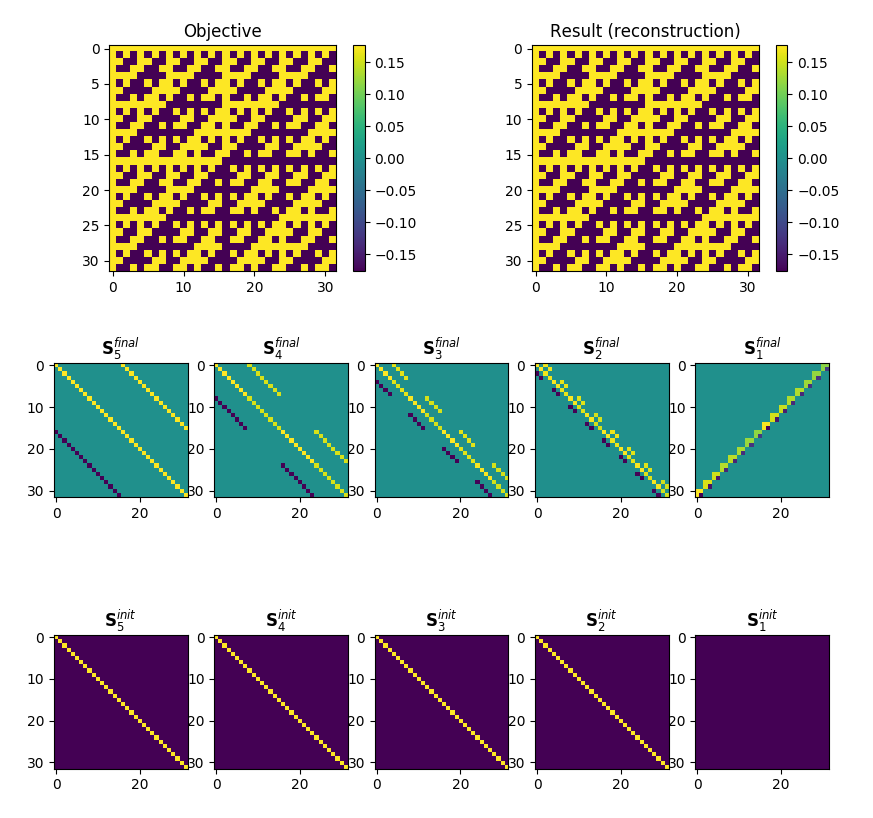
\includegraphics[scale=.4]{hadamard_decomposition.png}
 \caption{Decomposition of hadamard matrix by sparse factors. Bottom line show the initialization of the factors while middle line shows their final form at the end of the algorithm.}
\end{figure}


The complexity analysis is proposed under the following assumptions, which are satisfied in the mentioned applications and experiments: the number of factors is $\nfactors=\mathcal{O}\left (\log A\right )$; all but one sparse factors are of shape $A \times A$ and have $\bigO{A}$ non-zero entries while one of them is of shape $A\times B$ or $B\times A$ with $\bigO{B}$ non-zero entries.
In such conditions, the complexity of each line is:
\begin{itemize}
 \item [Lines~\ref{line:palm:init:lambda}-\ref{line:palm:normalize:S1}] Computing these normalization steps is linear in the number of non-zeros coefficients in $\rmS_1$.
 \item [Lines~\ref{line:palm:L}-\ref{line:palm:R}] Fast operators $\rmL$ and $\rmR$ are defined for subsequent use without computing explicitly the product.
 \item [Line~\ref{line:palm:c}] The spectral norm of $\rmL$ and $\rmR$ is obtained via a power method by iteratively applying each operator, benefiting from the fast transform.
 \item [Line~\ref{line:palm:D}] The cost of the gradient step is dominated by the product of sparse matrices.
\item [Line~\ref{line:palm:update:S}] The projection onto a sparse-constraint set takes $\bigO{A^2\log A}$ for all the $A\times A$ matrices and $\bigO{AB\log B}$ for the rectangular matrix at the leftmost or the rightmost position.
 \item [Line~\ref{line:palm:U}] The reconstructed matrix $\hat \rmU$ is computed using $\bigO{\log A}$ products between $A\times A$ sparse matrices, in $\bigO{A^2}$ operations each, and one product with a sparse matrix in $\bigO{AB}$.
 \item [Line~\ref{line:palm:update:lambda}] The numerator and denominator can be computed using a Hadamard product between the matrices followed by a sum over all the entries.
  \item [Line~\ref{line:palm:postprocess:S1}] Computing renormalization step is linear in the number of non-zeros coefficients in $\rmS_1$.
\end{itemize}

Hence, the overal time complexity of \palm is in $\bigO{AB\left (\log^2 A+\log B\right )}$, due to Lines~\ref{line:palm:D} and~\ref{line:palm:update:S}.

\section{Datasets}
\label{supp:datasets}

Table~\ref{table:data} provides some statistics about the used datasets.

\begin{table*}[!h]
\centering
\begin{tabular}{|c|c|c|c|c|c|}
\hline
\textbf{Dataset} & \textbf{Data dim.} $\datadim$        & \textbf{\# classes} & \textbf{Training set size} $\nexamples$ & \textbf{Test set size} $\nexamples'$ \\ \hline
MNIST                   & 784   & 10        & 60 000    & 10 000               \\ \hline
Fashion-MNIST           & 784   & 10        & 60 000    & 10 000               \\ \hline
% LFW                     & 1850  & 2529      & 8866      & N/A               \\ \hline
Blobs (clusters std: 12)   & 2000  & 1000      & 29000      & 1000               \\ \hline
Caltech256              & 2352  & 256      & 19952      & 9828               \\ \hline
\end{tabular}
\caption{Datasets statistics}
\label{table:data}
\end{table*}

\section{Sparse-factorization speed}
\label{seq:sparse_factor_benchmarking}
While more efficient implementations may be beneficial for larger deployment, our implementation is sufficient as a proof of concept for assessing the performance of the proposed approach. 
In particular, the running times of fast operators of the form $\prod_{q\in\intint{\nfactors}}{\rmS_q}$ have been measured when applying to random vectors, for several sparsity levels: 
as shown in Figure~\ref{fig:time_csr}, they are significantly faster than dense operators -- implemented as a \texttt{numpy.ndarray} matrix --, especially when the data size is larger than $10^3$.
\begin{figure}[tbh]
\centering
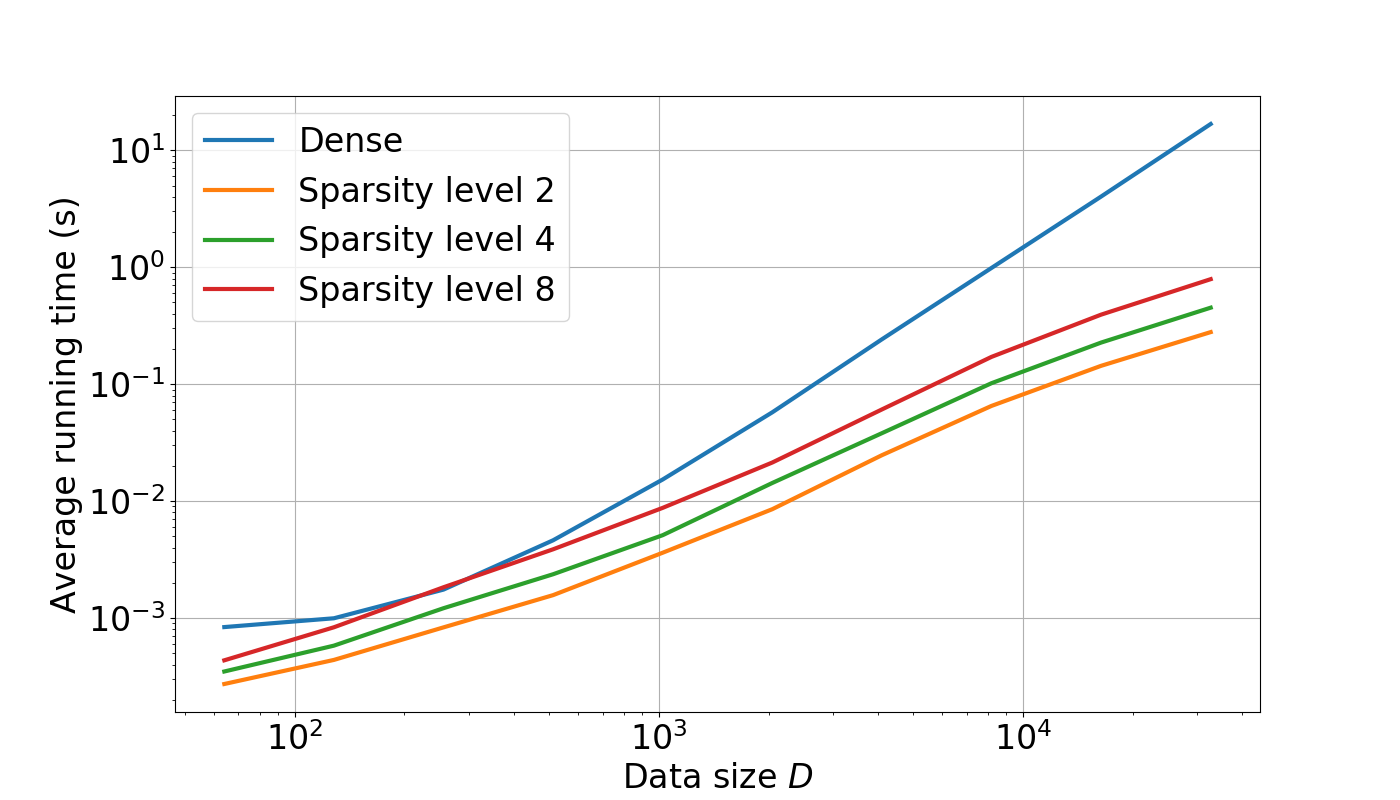
\includegraphics[width=.47\textwidth]{RunningTime4VaryingSparsity.png}
\caption{Running times, averaged over 30 runs, when applying dense or fast $\datadim \times \datadim$ operators to a set of 100 random vectors. The number of factors in fast operators equals $\log_2\left (\datadim\right )$ and the sparsity level denotes the number of non-zero coefficients per row and per column in each factor.}
\label{fig:time_csr}
\end{figure}

\section{Hierarchical-Palm4MSA}
\label{supp:hierarchical}

The Hierarchical-\palm algorithm has been used only for initialization of centroid sparse factors because it didn't improve that much the results when used on all iterations of  \qkmeans while it was very time consuming. Figure~\ref{fig:hierarchical_objective} shows the evolution of the objective function and the final centroids images when using the hierarchical version in all iteration.


\begin{figure*}[h]
\label{fig:hierarchical_objective}
\begin{subfigure}{.49\textwidth}
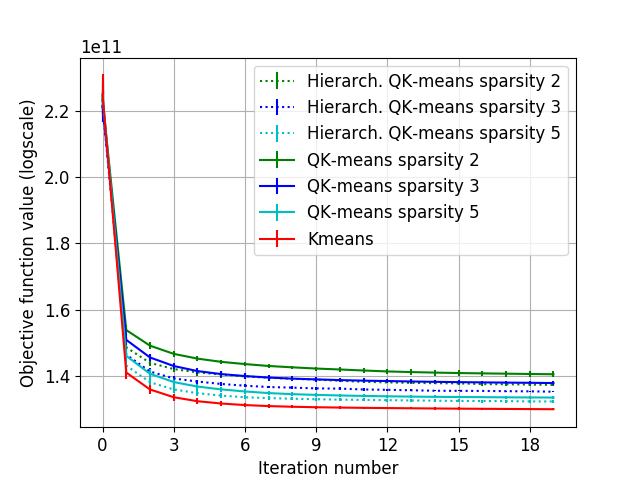
\includegraphics[width=\textwidth]{mnist30_objective_with_hierarchical.png}
\caption{MNIST, $\nclusters=30$: objective function.}
\label{fig:mnist:objfunhier}
\end{subfigure}
\begin{subfigure}{.49\textwidth}
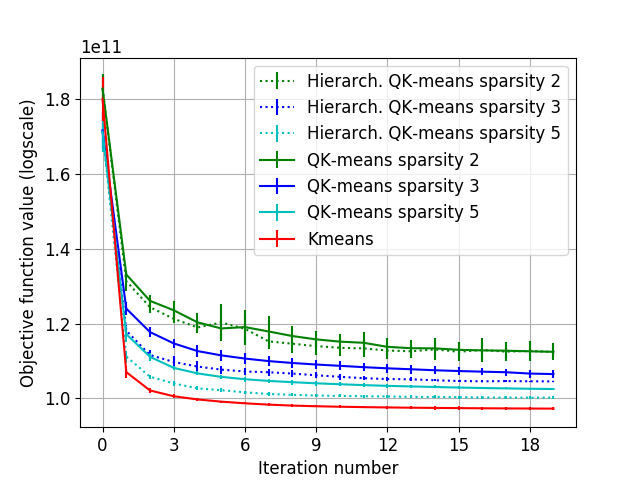
\includegraphics[width=\textwidth]{fashmnist30_objective_with_hierarchical.png}
\caption{Fashion-MNIST, $\nclusters=30$: objective function.}
\label{fig:fmnist:objfunhier}
\end{subfigure}
\begin{subfigure}{.49\textwidth}
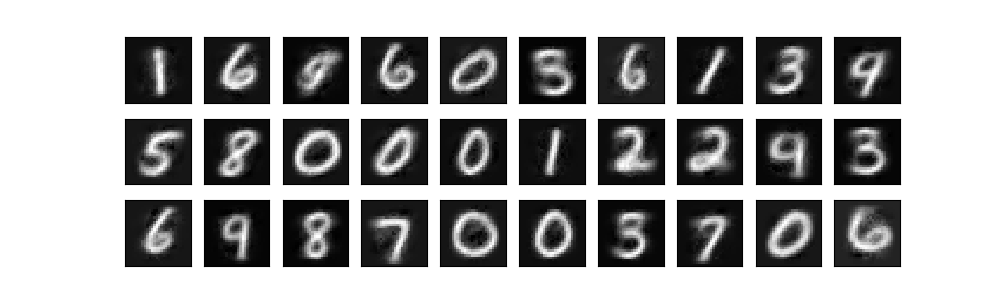
\includegraphics[width=\textwidth]{mnist30_hqkmeans_centroids.png}
\caption{Hierarchical-\palm \qkmeans centers.}
\label{fig:mnist:hqkmeans:centers}
\end{subfigure}
\begin{subfigure}{.49\textwidth}
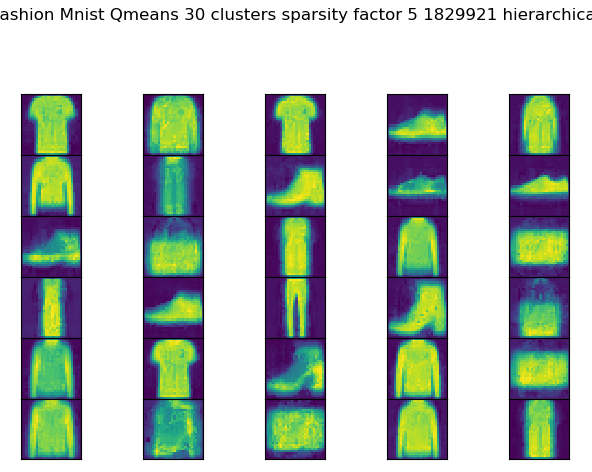
\includegraphics[width=\textwidth]{fashmnist30_hqkmeans_centroids.png}
\caption{Hierarchical-\palm \qkmeans centers.}
\label{fig:fmnist:hqkmeans:centers}
\end{subfigure}
\caption{Clustering results on MNIST (left) and Fashion-MNIST (right) for $\nclusters=30$ clusters. Results marked as ``hierarchical'' refers to the one obtained with hierarchical-\palm usage inside of the  \qkmeans algorithm}
\end{figure*}

\FloatBarrier

\section{Nyström approximation}
\label{supp:nystrom}

Nystr\"om approximation results: approximation accuracy (left) and running times (right). The uniform sampling based Nyström approximation running times are not displayed because they are the same as for the Nyström approximation based on \kmeans centers. Every experiment results are averaged over 5 runs. The vertical black lines are the standard deviation w.r.t. the runs. Numbers on top of each bar shows the number of parameter.
Results are shown in an histogram form rather than table for clearer interpretation. The \qkmeans approach gives better reconstruction error than the Nyström method based on uniform sampling although it is slightly worse than the one obtained with the regular \kmeans centers. We see that that the difference in approximation error between \kmeans and \qkmeans is almost negligible when compared to the approximation error obtained with the uniform sampling scheme.


We show the approximation error of the Nyström approximation based on different sampling schemes w.r.t. the real kernel matrix. This error is computed by the Froebenius norm of the difference between the matrices and then normalized:
\begin{equation}
 error = \frac{||\rmK - \tilde\rmK||_F}{||\rmK||_F}.
\end{equation}


\subsection{\texttt{Blobs}           }
\begin{figure*}[h]
\begin{subfigure}[]{.49\textwidth}
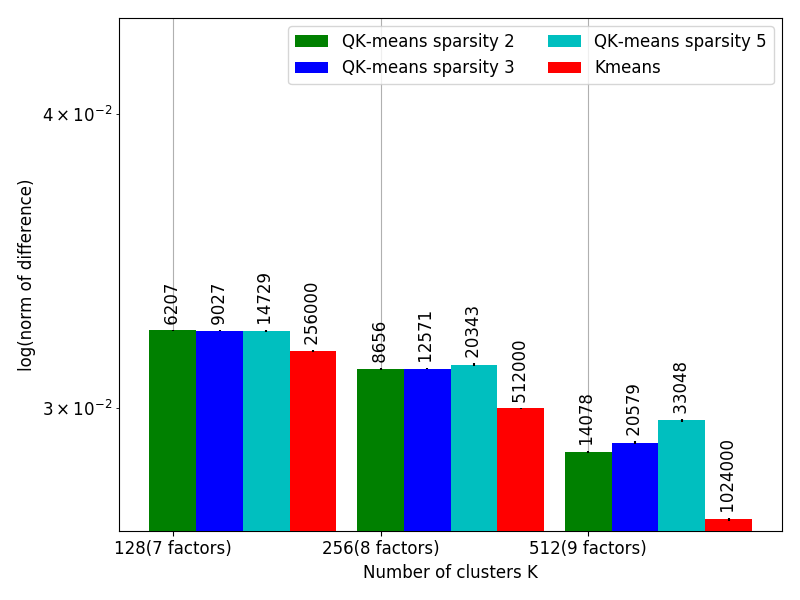
\includegraphics[width=\textwidth]{blobs_nystrom_error.png}
\caption{\texttt{Blobs}: Nyström reconstruction error.}
\label{fig:blobs:nystrom_error}
\end{subfigure}
\begin{subfigure}[]{.49\textwidth}
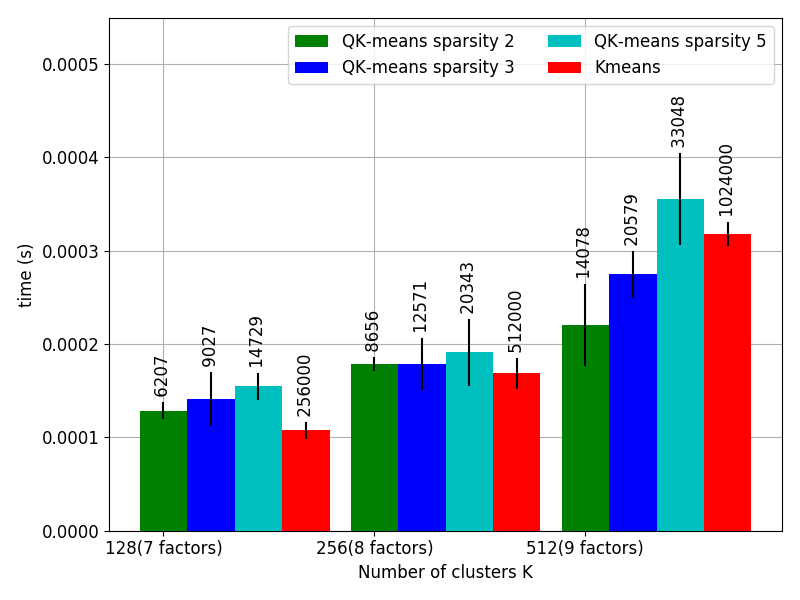
\includegraphics[width=\textwidth]{blobs_nystrom_inference_time.png}
\caption{\texttt{Blobs}: Nyström inference time.}
\label{fig:blobs:nystrom_time}
\end{subfigure}
\end{figure*}
\FloatBarrier
\subsection{\texttt{Mnist}           }
\begin{figure*}[h]
\begin{subfigure}[]{.49\textwidth}
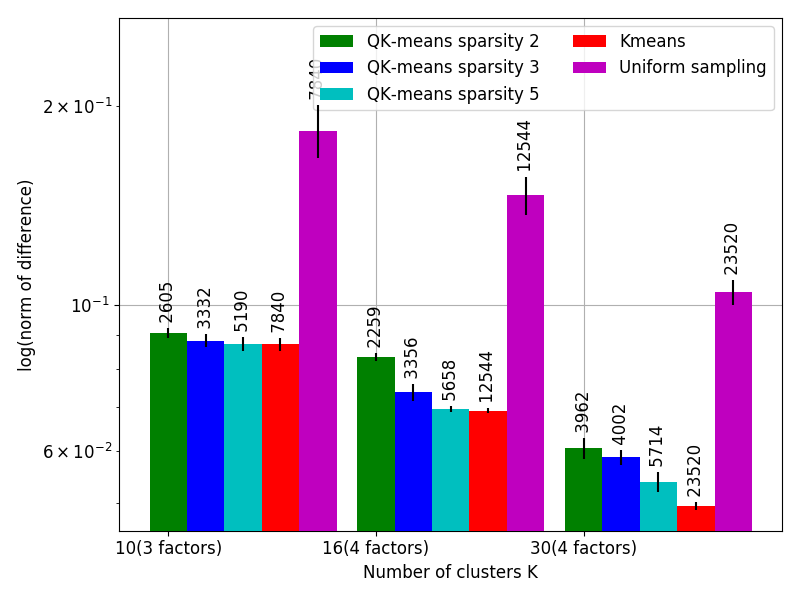
\includegraphics[width=\textwidth]{mnist_nystrom_error.png}
\caption{\texttt{MNIST}: Nyström reconstruction error.}
\label{fig:mnist:nystrom_error}
\end{subfigure}
\begin{subfigure}[]{.49\textwidth}
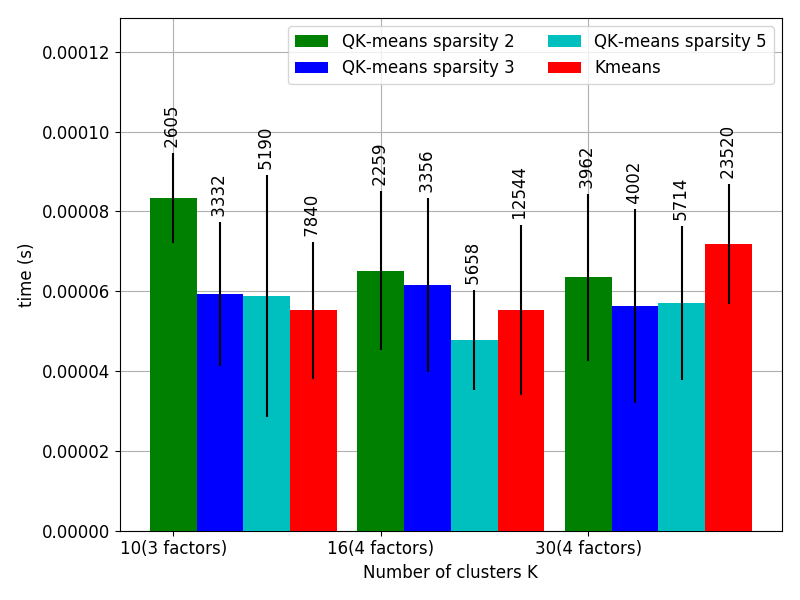
\includegraphics[width=\textwidth]{mnist_nystrom_inference_time.png}
\caption{\texttt{MNIST}: Nyström inference time.}
\label{fig:mnist:nystrom_time}
\end{subfigure}
\end{figure*}
\FloatBarrier
\subsection{\texttt{Fashion-MNIST}}
\begin{figure*}[h]
 \begin{subfigure}[]{.49\textwidth}
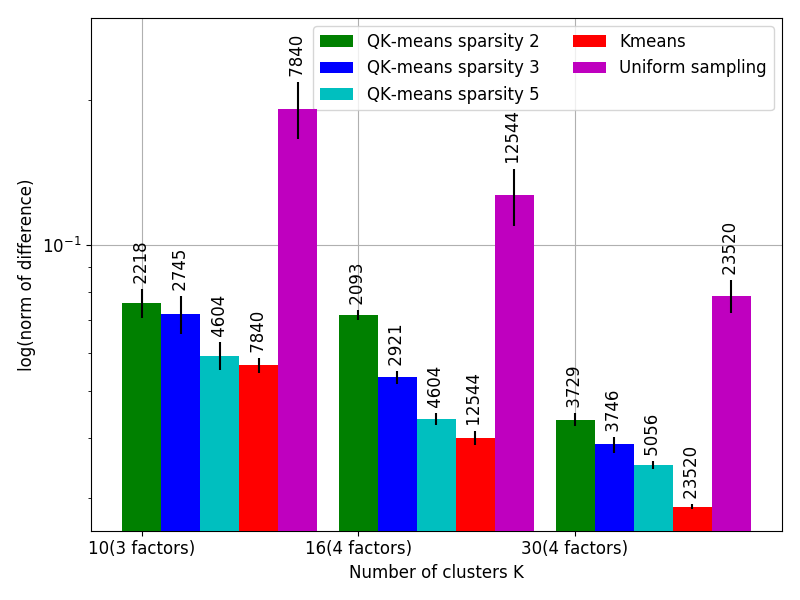
\includegraphics[width=\textwidth]{fashmnist_nystrom_error.png}
\caption{\texttt{Fashion-MNIST}: Nyström reconstruction error.}
\label{fig:fashmnist:nystrom_error}
\end{subfigure}
\begin{subfigure}[]{.49\textwidth}
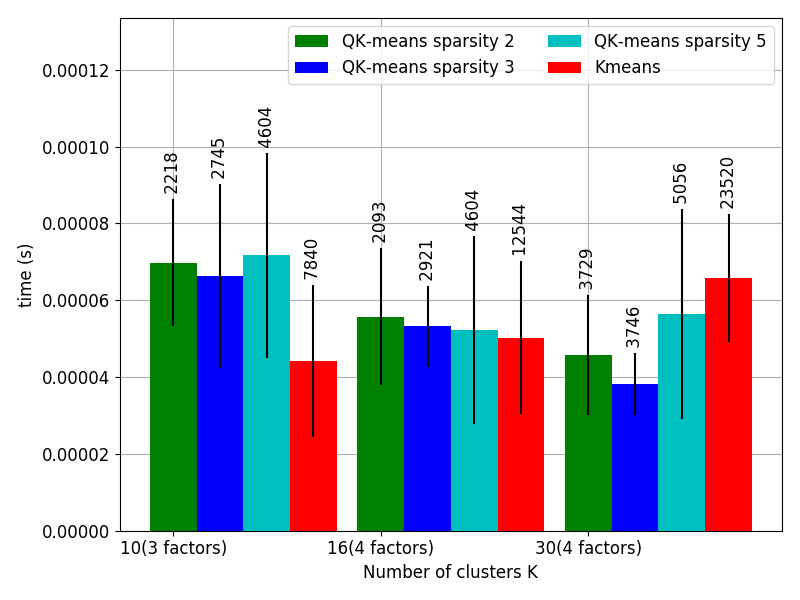
\includegraphics[width=\textwidth]{fashmnist_nystrom_inference_time.png}
\caption{\texttt{Fashion-MNIST}: Nyström inference time.}
\label{fig:fashmnist:nystrom_time}
\end{subfigure}
\end{figure*}
\FloatBarrier
\subsection{\texttt{Caltech256}      }
\begin{figure*}[h]
\begin{subfigure}[]{.49\textwidth}
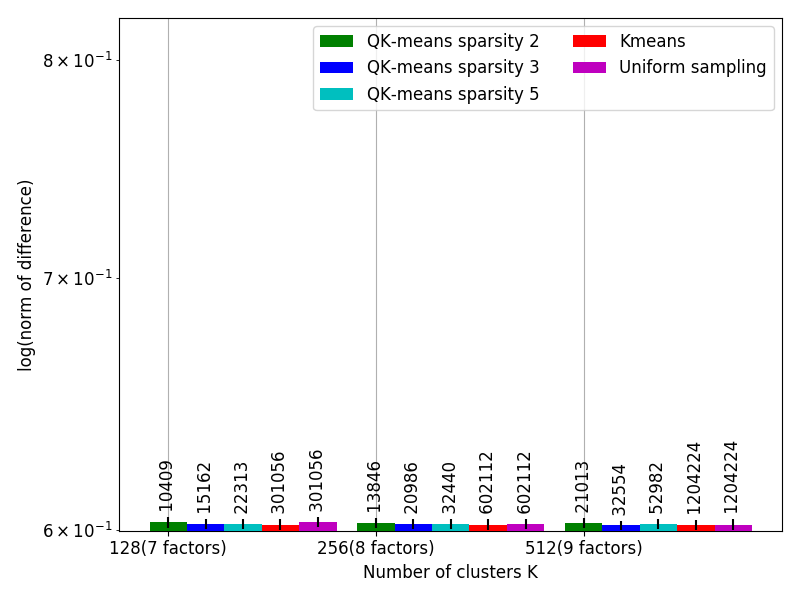
\includegraphics[width=\textwidth]{caltech_nystrom_error.png}
\caption{\texttt{Caltech256}: Nyström reconstruction error.}
\label{fig:caltech:nystrom_error}
\end{subfigure}
\begin{subfigure}[]{.49\textwidth}
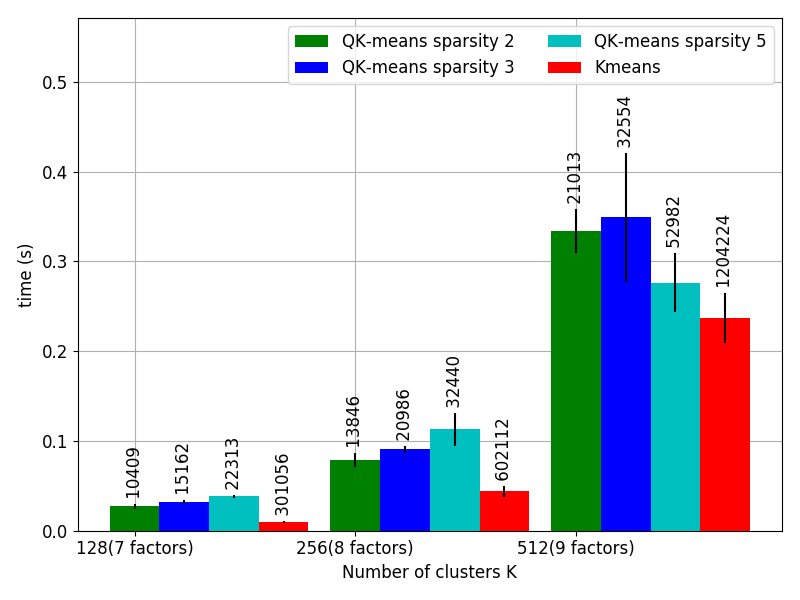
\includegraphics[width=\textwidth]{caltech_nystrom_inference_time.png}
\caption{\texttt{Caltech256}: Nyström inference time.}
\label{fig:caltech:nystrom_time}
\end{subfigure}
\end{figure*}


\todo[inline]{Faire un supplementary material montrant les expériences préliminaires de gain potentiel de temps lors de l'entrainement pour le jeu de données énorme}

\todo[inline]{Ajouter le déroulement de l'equation (equation 8 environ) centers update step dans les supplementary materials}

\todo[inline]{supplementary material montrant l'impact de la sparsity factor}







